\documentclass{article}
\usepackage[utf8x]{inputenc}
\usepackage[english]{babel}

%Math symbols
\usepackage{amsmath}
\usepackage{amssymb}
\let\oldPr\Pr
\renewcommand{\Pr}[1]{\text{Pr} \left( #1 \right)}
\newcommand{\E}[1]{\mathbb{E} \left[ #1 \right]}
\newcommand{\argmin}[2]{\underset{#1}{\arg \min} \left\{ #2 \right\}}
\newcommand{\fancyS}{\mathcal{S}}
\newcommand{\fancyA}{\mathcal{A}}
\newcommand{\R}{\mathbb{R}}
\newcommand{\N}{\mathbb{N}}
\newcommand{\rev}{\textit{REV}}
\newcommand{\orgmdp}{\text{MDP}_\text{Org}}
\newcommand{\auxmdp}{\text{MDP}_\text{RandStop}}
\newcommand{\revorg}{\textit{REV}_\text{Org}}
\newcommand{\revaux}{\textit{REV}_\text{RandStop}}
\newcommand{\termaux}{\textit{Term}_\text{RandStop}}

%Theorems
\usepackage{amsthm}
\newtheorem{definition}{Definition}
\newtheorem{theorem}{Theorem}
\newtheorem{corollary}[theorem]{Corollary}
\newtheorem{lemma}[theorem]{Lemma}
\newtheorem{assumption}{Assumption}

%Figures
\usepackage{graphicx}
\usepackage{float}

%Bibliography
\usepackage{natbib}
\makeatletter
\renewcommand{\@biblabel}[1]{[#1]\hfill}
\makeatother

%Title
\title{MDP Analysis for Blockchain}
\author{Roi Bar Zur \and Ittay Eyal \and Aviv Tamar}
\date{}

\begin{document}

\maketitle

\begin{abstract}
    TODO: Add abstract
\end{abstract}

\section{Introduction}

\subsection{}
TODO: Intro

\subsection{Contributions}
The contributions of the paper are as follows:
\begin{enumerate}
    \item Designing a novel method to solve Blockchain protocols modeled as MDPs
    \item Proved the new method converges to the optimal solution and bounded the approximation error.
    \item Recreated the approximately optimal results of \cite{sapirshtein2016optimal} for Bitcoin.
    \item Surpassed the results of \cite{hou2019squirrl} for Ethereum.
    \item Analyzed the new method's running time and showed it is more efficient than the current state of the art method (\cite{sapirshtein2016optimal}).
    \item Empirical analysis of the trade-off between running time and approximation error.
\end{enumerate}

TODO: Add navigation paragraph

\section{Related Work}
Eyal and Sirer were the first to show that the Bitcoin protocol is not incentive compatible (\cite{eyalmajority}). They have demonstrated and analyzed a strategy (called selfish mining or SM1) which can be used by miners and yields higher rewards than acting honestly. Selfish mining involves withholding newly minted blocks and violating the longest chain rule. The existence of such a strategy rules out the honest protocol as a Nash equilibrium.

The analysis in \cite{eyalmajority} gives a closed form formula of the revenue a miner can get if she uses SM1 and the minimal threshold for the relative computation power an attacker need such that using SM1 is superior to following the protocol. However, the analysis does not guarantee that an attacker with a relative power lower than the threshold cannot deviate in some other way and profit. This means that the SM1 threshold is an upper bound on the security threshold of the protocol. Overall, this analysis implies that under the reasonable assumption of $\gamma = 0.5$ the security threshold of Bitcoin is 0.25 at most.

Sapirshtein et al.~modeled the Bitcoin protocol as an MDP (Markov Decision Process, described in \ref{MDP_explain}) and solved the MDP in order to obtain approximately optimal strategies (\cite{sapirshtein2016optimal}). Their analysis yields an accurate approximation of the security threshold of Bitcoin. For example, they found that for some parameters, the threshold is as low as 0.231. 

Other works have tried to generalize the SM1 strategy to Ethereum and analyze its revenue in order to get an upper bound on the security threshold of Ethereum (\cite{ritz2018impact}, \cite{feng2019selfish}, \cite{grunspan2019selfish}). \cite{ritz2018impact} used a Monte-Carlo simulation in order to assess the revenue of their generalized SM1 strategy while \cite{feng2019selfish} and \cite{grunspan2019selfish} used a theoretical analysis. Nevertheless, all of these works analyze a specific strategy and therefore can only strive to obtain an upper bound of the security threshold.

A recent work by Charlie Hou, Mingxun Zhou and others demonstrates a new technique (called SquirRL) to analyze blockchain protocols (\cite{hou2019squirrl}). This method is based on the method of \cite{sapirshtein2016optimal} but instead of using MDPs in they use Q-learning. This is a similar method which allows using neural networks. SquirRL was used for Bitcoin and Ethereum and obtained a better upper bound for the security threshold of Ethereum.  By observing the results for bitcoin and comparing to \cite{sapirshtein2016optimal}, they deduce that their method typically finds solutions with revenues approximately 1-2\% lower than the optimum. Due to the approximation in their method, the threshold they find is not guaranteed to be approximately correct but only an upper bound.

\section{Name TBD}
TODO: Think of a name for the method (Random stop etc.)\\
Random Stop\\
Slot Machine\\
Ratio Reformation\\
Denominator Ironing/Smoothing\\

\subsection{Motivation}
Sapirshtein et al.~ (\cite{sapirshtein2016optimal}) modeled the Bitcoin protocol as an MDP with an objective function of the form:
\begin{gather*}
    \rev = \E{\lim\limits_{T\to\infty} \frac{\sum\limits_{t=1}^T R_t^1}{\sum\limits_{t=1}^T R_t^1 + R_t^2}}
\end{gather*}
Where $R_t^1$ is the attacker's reward at step $t$ and $R_t^2$ is the reward of the rest of the network at step $t$.

This form is not standard since it is not linear in the reward at each stage. In order to overcome this issue they show a novel technique of transforming this MDP to a standard linear reward MDP of the form:
\begin{gather*}
    \textit{REV}(\rho) = \E{\lim\limits_{T\to\infty} \sum\limits_{t=1}^T (1 - \rho) \cdot R_t^1 + \rho \cdot R_t^2}
\end{gather*}
Their method involves a binary search over $\rho \in [0,1]$ and solving the transformed MDP for the a given $\rho$ at every stage.
This method yields a close approximation but is computationally expensive due to the binary search.

This paper describes an alternative way to transform the MDP to a linear form which does not require a binary search at all. Using the new method, solving the MDP only once suffices.

\subsection{Markov Decision Process}\label{MDP_explain}
A Markov decision process (MDP) is a type of a controlled stochastic process \cite{bertsekas1995dynamic}. The process is comprised of an agent (in this paper, also known as the attacker) who has a set of actions $\fancyA$ and the environment which has a set of states $\fancyS$.
The game goes as follows: at every step $t$, the agent observes the environment's state $s \in \fancyS$ and decides to take some action $a \in \fancyA$. Then, the environment transitions stochastically to a new state $s' \in \fancyS$, the agent is awarded some $R_t = R_a(s, s')$ and the next step is played.

The transitions between states are Markovian, meaning that the distribution of the next state depends only on the current state and the agent's action. Formally:
\begin{gather*}
   \Pr{s_{i+1} = s' | s_i = s, a_i = a} =  P_a(s, s')
\end{gather*}
where $s_i$ and $a_i$ are the state and chosen action at step $i$ respectively.

The agent's policy is a mapping from the state space to the action space which given a state of the process, gives the action the agent takes. An MDP with a specific policy induces a Markov chain since at each state the action taken is determined by the policy. The agent wishes to maximize an objective function of some form linear in the step rewards. A relevant standard objective is the discounted reward criterion:
\begin{gather*}
	R = \E{\lim\limits_{T \to \infty} \sum\limits_{t=0}^T \beta^t R_t}
\end{gather*}
Note that $\fancyS, \fancyA$ and the functions $P_a(s, s'), R_a(s, s')$ are fully known to the agent.

There are standard algorithms for solving MDPs such as value Iteration and Q-learning. Both methods find an approximately optimal policy given an MDP and converge to the optimum as they are allowed to run more time.
Value iteration requires  $P_a(s, s')$ and $R_a(s, s')$ explicitly.
Q-learning is somewhat similar to value iteration but instead of requiring $P_a(s, s')$ and $R_a(s, s')$ explicitly it learns them. In addition, Q-Learning can work with a large state space by using function approximation, e.g., neural networks.

\subsection{Method}
Given an MDP of a blockchain protocol, w.l.o.g, the agent's objective function which she wants to maximize can be defined as:
\begin{gather*}
   \rev = \E{\lim\limits_{T\to\infty} \frac{\sum\limits_{t=1}^T R_t}{\sum\limits_{t=1}^T D_t}}
\end{gather*}
Where $R_t$ is the reward the miner receives in step $t$ and $D_t$ is the contribution of the step $t$ towards the difficulty adjustment.

In Bitcoin for example, the difficulty contribution is the sum of rewards all parties receive. Thus $\rev_a$ is equivalent to the relative revenue of the miner. In Ethereum, the difficulty contribution in step $t$ is the amount of the amount of blocks added to the main chain and as uncles. This is since in Ethereum uncle blocks are also considered for the difficulty adjustment. This target function is non-linear in the rewards and therefore standard MDP solution methods will not work.

The method of solving an MDP of this form consists of two stages:
\begin{enumerate}
    \item Constructing an auxiliary MDP (marked by $\auxmdp$) based on the original MDP (marked by $\orgmdp$). $\auxmdp$ has the same state space $\orgmdp$ and is essentially a duplicate of $\orgmdp$. But $\auxmdp$ is constructed such that every transition in it has some chance to end the process and move to a finite state. If this does not happen then the transition occurs as in $\orgmdp$.
    At every transition, the chance to end abruptly is $(1 - \frac{1}{D})^{D_t}$ where $D$ is some chosen parameter.\\
    The objective function of $\auxmdp$ is:
    \begin{gather*}
        \revaux = \E{\frac{1}{D} \sum\limits_{t=0}^\text{Term} R_t}
    \end{gather*}
    where Term is a random variable indicating the step in which the process terminates. This is practically a discounted reward with $\beta = 1$ and setting $R_t = 0$ for all $t > \text{Term}$.
    \item Solving $\auxmdp$ using standard MDP solver algorithms (e.g. Value Iteration) to obtain an approximately optimal policy.
\end{enumerate}

Note that the chance to end the process abruptly depends on $D_t$ and the higher $D_t$ is, the higher the chance to end the process. Intuitively, this encourages consideration of how actions add to the difficulty contribution and finding a balance between the reward added and the difficulty contribution. $D$ is called the expected horizon since this is the expected total difficulty contribution when the process ends (this will be proved formally later on).

Then, in order to analyze the revenue of the policy one has to calculate the steady-state  distribution of the Markov chain induced by the policy in $\orgmdp$. Then, use the steady-state probability distribution to calculate the expected reward and expected difficulty contribution of each step. The revenue is then the ratio between the two values.

\subsection{Proof of Optimality}
\begin{definition}
    Denote the revenue of the attacker in $\orgmdp$ as:
    \begin{gather*}
        \revorg \triangleq \E{\lim\limits_{T\to\infty} \frac{\sum\limits_{t=1}^T R_t}{\sum\limits_{t=1}^T D_t}}
    \end{gather*}
\end{definition}
\begin{definition}
    At every step $t$, $X_t$ is a random variable indicating whether the process $\auxmdp$ terminated at this step. It is defined as:
    \begin{gather*}
        X_t \triangleq
        \begin{cases}
            1 & \text{w.p } \left( 1 -\frac{1}{D} \right)^{D_t} \text{ (continue)} \\
            0 & \text{w.p } 1 - \left( 1 -\frac{1}{D} \right)^{D_t} \text{ (stop)} \\
            \end{cases}
    \end{gather*}
\end{definition}
\begin{definition}
    The step in which $\auxmdp$ terminates is defined as:
    \begin{gather*}
        \termaux(D) \triangleq \arg \min\limits_T \{ X_T = 0 \}
    \end{gather*}
\end{definition}
\begin{definition}
    The revenue of the attacker in the linear reward MDP we defined is:
    \begin{gather*}
         \revaux(D) \triangleq \lim\limits_{D\to\infty} \E{\frac{1}{D}\sum\limits_{t=1}^{\termaux(D)} R_t}
    \end{gather*}
\end{definition}
\begin{theorem}
    Optimizing the original MDP is the same as optimizing the auxiliary MDP constructed by the method.
    \begin{gather*}
        \revorg = \lim\limits_{D\to\infty}  \revaux(D)
    \end{gather*}
\end{theorem}

% Proofs
TODO: Reorganize proofs, remove redundancies and change name of MDP and MDP'.

Using the notations of \cite{white2001markov}, $X_n$ denotes a Markov chain in general.
$X_n$ may also denote a random variable of the state of the Markov chain at time $n$.
$S$ denotes the state space of the Markov chain.
$P$ denotes the transition matrix.

An irreducible chain is a chain in which for every pair of states $i$ and $j$ there is a chance to transition from $i$ to $j$ after any number of steps.

\begin{definition}
    (Definition 25 p. 16 \cite{white2001markov}) \\
    A hitting time of a state $i$ by a process $X_n$ is defined by:
    \begin{gather*}
        \tau_i = \min \{ n \geq 2 : X_1 = X_n = i \}
    \end{gather*}
\end{definition}
Intuitively, the hitting time of a state is a random variable of the number of steps it takes to enter the state when starting at said state.

A positive recurrent state  is a state $i$ for which the expected hitting time is finite.

A period of a state is the gcd of all possible values for its hitting time.
A state is aperiodic if its period is 1.

For an irreducible chain, if one state is positive recurrent and aperiodic then all its states are. In addition, the chain is called positive recurrent and aperiodic.

\begin{lemma}\label{prop69}
    (Proposition 69 p. 44 \cite{white2001markov}) \\
    Let $X_n$ be an irreducible positive recurrent Markov chain with stationary distribution $\pi$.
    Suppose $V_n$, $n \geq 1$, are real-valued random variables associated with the chain such that \\
    \begin{gather*}
        \E{V_n|X_1,X_2,...,X_n} = a_{X_n}, \ \ \ n \geq 1
    \end{gather*}
    where $a_j$ are constants. Then, for the hitting time $\tau_i$ of a fixed state $i$,
    \begin{gather*}
        \E{\sum\limits_{n=1}^{\tau_i - 1} V_n \middle\vert X_1 = i} = \frac{1}{\pi_i} \sum\limits_{j \in S} a_j \pi_j
    \end{gather*}
    provided the last sum is absolutely convergent.
\end{lemma}
This lemma gives a way to calculate the expected cumulative sum of a random variable which depends on the current state of the chain until some chosen state is entered. For example, in Bitcoin, $V_n$ can be the number of blocks the attacker adds to the chain at step $n$. This variable clearly depends on the state and its expected value is a function of the state.

\begin{lemma}\label{cor79}
    (Corollary 79 p. 50 \cite{white2001markov}) \\
    For a fixed integer $\ell$, the process $\tilde{X}_n = (X_n,...,X_{n+\ell})$ is an ergodic Markov chain on $S^{\ell + 1}$ with stationary distribution
    \begin{gather*}
        \pi(i) = \pi_{i_0} p_{i_0,i_1} \cdot \cdot \cdot p_{i_{\ell - 1}, i_\ell}
    \end{gather*}
    Hence, for $f:S^{\ell + 1} \to \R$,
    \begin{gather*}
        \lim\limits_{n \to \infty} n^{-1} \sum\limits_{m=1}^n f(\tilde{X}_m) = \sum\limits_{i \in S^{\ell + 1}} f(i) \pi(i) \ \ \ \text{a.s.},
    \end{gather*}
    provided the sum is absolutely convergent.
\end{lemma}
This lemma is a generalization of Lemma \ref{prop69}. First, instead of a random variable which depends on a single state, it allows using any (deterministic) function of the last $(\ell + 1)$ states. This is a powerful notion since it depends on multiple states instead of one.
Second, instead of cumulative sum until entering a said state, it provides the average of the function when the chain plays indefinitely.

\begin{lemma}\label{limiting_thm111_original}
    (Theorem 111 p. 74 \cite{white2001markov}) \\
    If $X_n$ is an ergodic Markov chain with stationary distribution $\pi$, then
    \begin{gather*}
        \sup_i |\Pr{X_n = i} - \pi_i| \to 0, \ \ \ \text{as } n \to \infty
    \end{gather*}
\end{lemma}
Intuitively, this means that any row of $P^n$ gets closer to $\pi$ as $n \to \infty$.
This is since for every $i, j$: $\Pr{X_n = i} = \sum\limits_{j \in S} \Pr{X_1 = j} \cdot (P^n)_{ji} \to \pi_i$. And this is for any choice of distribution for the initial state $X_1$.

Using the $L_1$ norm instead of $L_\infty$ and denoting the distribution of $X_1$ as $x$, the lemma can be rewritten:
\begin{lemma}\label{limiting_thm111}
    If $X_n$ is an ergodic Markov chain with stationary distribution $\pi$, then for any $\eta \in [0,1]^{|S|}$ such that $||\eta|| = 1$:
    \begin{gather*}
        \lim\limits_{n \to \infty} ||\eta P^n - \pi|| = 0
    \end{gather*}
\end{lemma}

From now on, we will assume a fixed policy $\sigma$. This means that any MDP we have can be reduced to a Markov chain by applying $\sigma$ to it.

\begin{definition}\label{ar_def}
    The absolute revenue of the attacker in the original MDP (under a specific policy) is:
    \begin{gather*}
        \rev \triangleq \E{\lim\limits_{T\to\infty} \frac{\sum\limits_{t=1}^T R_t}{\sum\limits_{t=1}^T D_t}}
    \end{gather*}
\end{definition}
$R_t$ is the reward of the attacker at step $t$ and $D_t$ is the difficulty contribution at step $t$.
For example, in Bitcoin $R_t$ would be the number of blocks the attacker adds to the main chain at step $t$ and $D_t$ would be the total number of blocks added to the main chain at said step (both blocks of the attacker and blocks of the rest of the network).

We make the easing assumption that at every step the maximal contribution to the difficulty is upper bounded by some constant $c$. Formally:
\begin{assumption}\label{assump_d_t_bounded}
    $\forall_t : 0 \leq D_t \leq c$
\end{assumption}

Reminder of the definition MDP': A replica of the original MDP where we also take every state and give it a chance to transition to the initial state and start over. This is denoted by $X_t$. The reward and difficulty contribution are the same as in the original. MDP' is determined by some chosen parameter $D$. \\
Denote the initial state of MDP and MDP' as $s_\text{init}$. \\
Denote $P_\sigma(i,j)$ as the chance to transition to state $j$ when the MDP is in state $i$ under policy $\sigma$. Denote $P'_\sigma(i,j)$ similarly for MDP'. Denote their steady-state distributions as $\pi_i$ and $\pi'_i$ respectively. \\
Also denote $R_\sigma(i,j)$ as the reward in MDP under policy $\sigma$ when transitioning from state $i$ to state $j$ and $D_\sigma(i,j)$ as the difficulty contribution in a similar manner. Note that $R_\sigma(i,j)$ and $D_\sigma(i,j)$ are equivalent in MDP and MDP'.

\begin{definition}\label{x_t_def}
    At every step $t$, $X_t$ is a random variable indicating whether MDP' terminated at this step. For some parameter $D \in \N$, it is defined as:
    \begin{gather*}
        X_t \triangleq
        \begin{cases}
            1 & \text{w.p } \left( 1 -\frac{1}{D} \right)^{D_t} \text{ (continue)} \\
            0 & \text{w.p } 1 - \left( 1 -\frac{1}{D} \right)^{D_t} \text{ (stop)} \\
        \end{cases}
    \end{gather*}
\end{definition}

\begin{corollary}\label{mdp_prime_transition_p}
    The transition probability of MDP' is:
    \begin{gather*}
        P'_\sigma(i,j) =
        \begin{cases}
            \left( 1 - \frac{1}{D} \right)^{D_\sigma(i,j)} P_\sigma(i,j) + 1 - \left( 1 - \frac{1}{D} \right)^{D_\sigma(i,j)} & j = s_\text{init} \\
            \left( 1 - \frac{1}{D} \right)^{D_\sigma(i,j)} P_\sigma(i,j) & \text{o.w}
        \end{cases}
    \end{gather*}
\end{corollary}

\begin{definition}\label{term_def}
    The step in which MDP' terminates is defined as:
    \begin{gather*}
        \termaux(D) \triangleq \argmin{T}{X_T = 0}
    \end{gather*}
\end{definition}
This is a random variable which denotes the first step in which "stop" is drawn.

\begin{definition}
    The absolute revenue of the attacker in MDP' we defined is:
    \begin{gather*}
         \revaux(D) \triangleq \frac{1}{D}\E{\sum\limits_{t=1}^{\termaux(D)} R_t}
    \end{gather*}
\end{definition}

MDP' is a function of $D$, any choice of $D$ would give a slightly different MDP'. We are interested at the behavior for a large enough $D$.
\begin{definition}\label{ar_prime_def} The limit of the absolute revenue as $D$ approaches $\infty$ is defines as $\revaux$. Formally:
    \begin{gather*}
          \triangleq \lim\limits_{D\to\infty} \revaux(D) = \lim\limits_{D\to\infty} \frac{1}{D}\E{\sum\limits_{t=1}^{\termaux(D)} R_t}
    \end{gather*}
\end{definition}

\begin{lemma}\label{diff_cont_lemma}
    The expected total contribution to the difficulty when MDP' terminates is asymptotically equivalent to $D$. Formally:
    \begin{gather*}
        \lim\limits_{D\to\infty} \frac{1}{D} \E{\sum\limits_{t=1}^{\termaux(D)} D_t} = 1
    \end{gather*}
\end{lemma}
This lemma is the reason we call $D$ the expected horizon. Intuitively, For a large enough $D$, the expected sum of the difficulty contribution from the start of the process until termination is close to $D$. This also explains the intuition behind the choice of AR' - instead of dividing by the actual difficulty contribution, we divide by the expected difficulty contribution.

\begin{proof}
    Define:
    \begin{gather*}
    \hat{X}_{ti} \triangleq
        \begin{cases}
            1 & \text{w.p } 1 -\frac{1}{D} \text{ (continue)} \\
            0 & \text{w.p } \frac{1}{D} \text{ (stop)} \\
        \end{cases},
        t \in \N, i \in [c]
    \end{gather*}
    Notice that from this definition and from definition \ref{x_t_def}, $X_t$ can be thought of as: $X_t = 1 \iff \forall_{i=1}^{D_t} \hat{X}_{ti} = 1$. Or in other words:
    \begin{gather}\label{x_t_decomp}
        X_t = \prod\limits_{i=1}^{D_t} \hat{X}_{ti}
    \end{gather}
    This decomposes each $X_t$ to be a function of a set of hidden i.i.d Bernoulli trials.
    Remember from definition \ref{term_def}:
    \begin{gather*}
        \termaux(D) = \argmin{T}{X_T = 0} = \argmin{T}{\prod\limits_{t=1}^T X_t = 0}
    \end{gather*}
    The last equivalence follows because for all $t < \termaux(D): X_t = 1$.\\
    By using \eqref{x_t_decomp}:
    \begin{gather*}
        \termaux(D) = \argmin{T}{\prod\limits_{t=1}^T \prod\limits_{i=1}^{D_t} \hat{X}_{ti} = 0}
    \end{gather*}
    Since all $\hat{X}_{ti}$ are i.i.d we can rename and renumber them as $\hat{Z}_j$ to get:
    \begin{gather*}
        \termaux(D) = \argmin{T}{\prod\limits_{j=1}^{\sum\limits_{t=1}^T D_t} \hat{Z}_j = 0}
    \end{gather*}
    Define:
    \begin{gather*}
        G = \argmin{k}{\prod\limits_{j=1}^{k} \hat{Z}_j= 0}
    \end{gather*}
    Notice since all $\hat{Z}_j$ are independent Bernoulli trials (continue means failure and stop means success). $G$ is distributed geometrically with a chance of success $p = \frac{1}{D}$. This yields:
    \begin{gather}\label{g_mean}
        \E{G} = \frac{1}{p} = D
    \end{gather}
    We will establish a relation between $\termaux(D)$ and $G$. Notice that by definition of $\termaux(D)$:
    \begin{gather}\label{term_is_t_1}
        \prod\limits_{j=1}^{\sum\limits_{t=1}^{\termaux(D)} D_t} \hat{Z}_j = 0
    \end{gather}
    \begin{gather}\label{term_is_t_2}
        \prod\limits_{j=1}^{\sum\limits_{t=1}^{\termaux(D)-1} D_t} \hat{Z}_j = 1
    \end{gather}
    The definition of $G$ and \eqref{term_is_t_1} yield:
    \begin{gather*}
        G \leq \sum\limits_{t=1}^{\termaux(D)} D_t
    \end{gather*}
    And \eqref{term_is_t_2} yields:
    \begin{gather*}
        G > \sum\limits_{t=1}^{\termaux(D)-1} D_t \geq \sum\limits_{t=1}^{\termaux(D)} D_t - c
    \end{gather*}
    The last inequality follows from assumption \ref{assump_d_t_bounded}.
    Overall:
    \begin{gather*}
        G \leq \sum\limits_{t=1}^{\termaux(D)} D_t < G + c \\
        \E{G} \leq \E{\sum\limits_{t=1}^{\termaux(D)} D_t} \leq \E{G} + c \\
        \frac{1}{D} \E{G} \leq \frac{1}{D} \E{\sum\limits_{t=1}^{\termaux(D)} D_t} \leq \frac{1}{D} (\E{G} + c) \\
        \lim\limits_{D \to \infty} \frac{1}{D} \E{G} \leq \lim\limits_{D \to \infty} \frac{1}{D} \E{\sum\limits_{t=1}^{\termaux(D)} D_t} \leq \lim\limits_{D \to \infty} \frac{1}{D} (\E{G} + c)
    \end{gather*}
    Swapping $\E{G}$ thanks to \eqref{g_mean}:
    \begin{gather*}
        1 = \lim\limits_{D \to \infty} \frac{1}{D} D \leq \lim\limits_{D \to \infty} \frac{1}{D} \E{\sum\limits_{t=1}^{\termaux(D)} D_t} \leq \lim\limits_{D \to \infty} \frac{1}{D} (D + c) = 1 \\
        \lim\limits_{D \to \infty} \frac{1}{D} \E{\sum\limits_{t=1}^{\termaux(D)} D_t} = 1
    \end{gather*}
\end{proof}

The main theorem:
\begin{theorem}\label{ar_ar_prime_eq}
    The absolute revenue of the MDP is equivalent to the absolute revenue of the MDP' (under the same policy):
    \begin{gather*}
        \revorg = \revaux
    \end{gather*}
\end{theorem}

First we make a few observations on MDP and MDP':
\begin{assumption}\label{assumption_irreducible}
    MDP and MDP' are irreducible.
\end{assumption}
This is true w.l.o.g because we can ignore all the states that are unreachable from $s_\text{init}$ and any transient states at the beginning.

\begin{lemma}\label{assumption_positive_recurrent}
    MDP and MDP' are positive recurrent.
\end{lemma}
\begin{proof}
     Since both are irreducible and $s_\text{init}$ is positive recurrent - in every state there is a chance to return to $s_\text{init}$ eventually. In MDP this is because $\alpha < 0.5$, the honest network will always catch up and the attacker cannot keep waiting forever, she must perform adopt at some point. In MDP' there is additionally a chance to go back to $s_\text{init}$. \\
\end{proof}

\begin{assumption}\label{assumption_aperiodic}
    MDP and MDP' are aperiodic.
\end{assumption}
We can say that both MDP and MDP' are aperiodic w.l.o.g because we can take any positive recurrent state and change it to have a chance to transition to itself with no reward and no difficulty contribution. This does not change AR or AR' at all since this just means that the game may halt for a few steps and then carry on normally. But, this change ensures the state has a period of 1 and with irreducibly this implies aperiodicity.

\begin{corollary}
    MDP and MDP' are ergodic.
\end{corollary}
This quickly follows from lemma \ref{assumption_positive_recurrent} and assumptions \ref{assumption_irreducible} and \ref{assumption_aperiodic}.

\begin{proof} (of the main theorem)\\
    Assume policy $\sigma$. \\
    Define the expected reward and difficulty contribution of every state, for MDP and MDP':
    \begin{gather*}
        \hat{R}_i = \sum\limits_{j \in S} R_\sigma(i,j)  P_\sigma(i,j)
    \end{gather*}
    \begin{gather*}
        \hat{R}'_i = \sum\limits_{j \in S} R_\sigma(i,j)  P'_\sigma(i,j)
    \end{gather*}
    \begin{gather*}
        \hat{D}_i = \sum\limits_{j \in S} D_\sigma(i,j)  P_\sigma(i,j)
    \end{gather*}
    \begin{gather*}
        \hat{D}'_i = \sum\limits_{j \in S} D_\sigma(i,j)  P'_\sigma(i,j)
    \end{gather*}
    These are the expected reward/difficulty contribution in MDP/MDP' when transitioning from state $i$. \\
    Remember from definition \ref{ar_def}:
    \begin{gather*}
        \revorg = \E{\lim\limits_{T\to\infty} \frac{\sum\limits_{t=1}^T R_t}{\sum\limits_{t=1}^T D_t}}
    \end{gather*}
    Let's analyze this expression first:
    \begin{gather*}
        \lim\limits_{T\to\infty} \frac{\sum\limits_{t=1}^T R_t}{\sum\limits_{t=1}^T D_t} =
        \frac{\lim\limits_{T\to\infty} \frac{1}{T} \sum\limits_{t=1}^T R_t}{\lim\limits_{T\to\infty} \frac{1}{T} \sum\limits_{t=1}^T D_t} = \frac{\sum\limits_{(i,j) \in S^2} R_\sigma(i,j) \pi_i P_\sigma(i,j)}{\sum\limits_{(i,j) \in S^2} D_\sigma(i,j) \pi_i P_\sigma(i,j)}
    \end{gather*}
    The first equality is true only if both limits are well defined and the denominator is not 0. We will see that this is indeed the case after fully developing the expression. \\
    The last equality follows from lemma \ref{cor79} with $\ell = 1$ when choosing \\
    $f: (X_t, X_{t+1}) \mapsto R_\sigma(X_t,X_{t+1})$ for the nominator and \\
    $f: (X_t, X_{t+1}) \mapsto D_\sigma(X_t,X_{t+1})$ for the denominator.\\
    By taking the sums apart we get:
    \begin{gather*}
        \frac{\sum\limits_{(i,j) \in S^2} R_\sigma(i,j) \pi_i P_\sigma(i,j)}{\sum\limits_{(i,j) \in S^2} D_\sigma(i,j) \pi_i P_\sigma(i,j)} = \frac{\sum\limits_{i \in s} \sum\limits_{j \in s} R_\sigma(i,j) \pi_i P_\sigma(i,j)}{\sum\limits_{i \in s} \sum\limits_{j \in s} D_\sigma(i,j) \pi_i P_\sigma(i,j)} = \frac{\sum\limits_{i \in s} \hat{R}_i \pi_i}{\sum\limits_{i \in s} \hat{D}_i \pi_i}
    \end{gather*}
    We get that the last expression is not random so its expectation is itself. Overall:
    \begin{gather*}
        \revorg = \E{\lim\limits_{T\to\infty} \frac{\sum\limits_{t=1}^T R_t}{\sum\limits_{t=1}^T D_t}} = \E{\frac{\sum\limits_{i \in s} \hat{R}_i \pi_i}{\sum\limits_{i \in s} \hat{D}_i \pi_i}} = \frac{\sum\limits_{i \in s} \hat{R}_i \pi_i}{\sum\limits_{i \in s} \hat{D}_i \pi_i}
    \end{gather*}
    The last equality follows from the fact that the expression in the expectation is constant. \\
    From definition \ref{ar_prime_def} and from lemma \ref{diff_cont_lemma}:
    \begin{gather*}
        \revaux = \lim\limits_{D\to\infty} \frac{1}{D}\E{\sum\limits_{t=1}^{\termaux(D)} R_t} = \frac{\lim\limits_{D\to\infty} \frac{1}{D}\E{\sum\limits_{t=1}^{\termaux(D)} R_t}}{{\lim\limits_{D\to\infty} \frac{1}{D} \E{\sum\limits_{t=1}^{\termaux(D)} D_t}}} = \\
        = \lim\limits_{D\to\infty} \frac{\E{\sum\limits_{t=1}^{\termaux(D)} R_t}}{{\E{\sum\limits_{t=1}^{\termaux(D)} D_t}}}
    \end{gather*}
    Note that:
    \begin{enumerate}
        \item $(\termaux(D) + 1)$ is the hitting time of $s_\text{init}$.
        \item In MDP', $\E{R_t | X_t = i} = \hat{R}'_i$ and $\E{D_t | X_t = i} = \hat{D}'_i$,
    \end{enumerate}
    Therefore lemma \ref{prop69} can be used (twice) to obtain:
    \begin{gather*}
        \revaux = \lim\limits_{D\to\infty} \frac{\E{\sum\limits_{t=1}^{\termaux(D)} R_t}}{{\E{\sum\limits_{t=1}^{\termaux(D)} D_t}}} = \lim\limits_{D\to\infty} \frac{(\pi'_{s_\text{init}})^{-1} \sum\limits_{i \in S} \hat{R}'_i \pi'_i}{(\pi'_{s_\text{init}})^{-1} \sum\limits_{i \in S} \hat{D}'_i \pi'_i} = \lim\limits_{D\to\infty} \frac{\sum\limits_{i \in S} \hat{R}'_i \pi'_i}{\sum\limits_{i \in S} \hat{D}'_i \pi'_i}
    \end{gather*}
    Remember from corollary \ref{mdp_prime_transition_p}:
    \begin{gather*}
        P'_\sigma(i,j) =
        \begin{cases}
            \left( 1 - \frac{1}{D} \right)^{D_\sigma(i,j)} P_\sigma(i,j) + 1 - \left( 1 - \frac{1}{D} \right)^{D_\sigma(i,j)} & j = s_\text{init} \\
            \left( 1 - \frac{1}{D} \right)^{D_\sigma(i,j)} P_\sigma(i,j) & \text{o.w}
        \end{cases}
    \end{gather*}
    Since $P_\sigma(i,j)$ and $D_\sigma(i,j)$ are independent of $D$ it is trivial ot see that:
    \begin{gather}\label{P_convergence}
        \forall i,j \in S: \lim\limits_{D \to \infty} P'_\sigma(i,j) = P_\sigma(i,j)
    \end{gather}
    It quickly follows that:
    \begin{gather*}
        \forall i \in S: \lim\limits_{D \to \infty} \hat{R}'_i = \hat{R}_i
    \end{gather*}
    \begin{gather*}
        \forall i \in S: \lim\limits_{D \to \infty} \hat{D}'_i = \hat{D}_i
    \end{gather*}
    In addition, since $\pi$ and $\pi'$ are the stationary distributions of MDP and MDP' respectively, by lemma \ref{limiting_thm111}:
    \begin{align*}
        \forall \eta \in [0,1]^{|S|} \text{s.t } ||\eta|| = 1: &
        \lim\limits_{n \to \infty} ||\eta P^n - \pi|| = 0 \\
        & \lim\limits_{n \to \infty} ||\eta (P')^n - \pi'|| = 0
    \end{align*}
    \eqref{P_convergence} implies:
    \begin{gather*}
        \lim\limits_{D \to \infty} P' = P
    \end{gather*}
    It is easy to see that for any $n$, it holds that:
    \begin{gather*}
        \lim\limits_{D \to \infty} (P')^n = P^n
    \end{gather*}
    Or in another form:
    \begin{gather*}
        \lim\limits_{D \to \infty} ||(P')^n - P^n|| = 0
    \end{gather*}
    By using the triangle inequality, we get:
    \begin{gather*}
        ||\pi' - \pi|| = ||\pi' - \eta (P')^n + \eta (P')^n - \eta P^n + \eta P^n - \pi|| \leq \\
        \leq ||\pi' - \eta (P')^n|| + ||\eta (P')^n - \eta P^n|| + ||\eta P^n - \pi||
    \end{gather*}
    Overall:
    \begin{gather*}
        \lim\limits_{D \to \infty} ||\pi' - \pi|| = \lim\limits_{D \to \infty} \lim\limits_{n \to \infty} ||\pi' - \pi|| \leq \\
        \leq \lim\limits_{D \to \infty} \lim\limits_{n \to \infty} ||\pi' - \eta (P')^n|| + ||\eta (P')^n - \eta P^n|| + ||\eta P^n - \pi|| = \\
        = \lim\limits_{D \to \infty} \lim\limits_{n \to \infty} ||\eta (P')^n - \eta P^n|| \leq \lim\limits_{D \to \infty} ||\eta (P')^{n_0} - \eta P^{n_0}|| = 0
    \end{gather*}
    The first equality follows from the fact that $\pi$ and $\pi'$ are independent of $n$.
    
    Using all limits and the fact that the sums are finite (because $S$ is finite), we can write:
    \begin{gather*}
        \revaux = \lim\limits_{D\to\infty} \frac{\sum\limits_{i \in S} \hat{R}'_i \pi'_i}{\sum\limits_{i \in S} \hat{D}'_i \pi'_i} = \frac{\sum\limits_{i \in S} \left( \lim\limits_{D\to\infty} \hat{R}'_i \right) \left( \lim\limits_{D\to\infty} \pi'_i \right)}{\sum\limits_{i \in S} \left( \lim\limits_{D\to\infty} \hat{D}'_i \right) \left( \lim\limits_{D\to\infty} \pi'_i \right)} = \\
        = \frac{\sum\limits_{i \in s} \hat{R}_i \pi_i}{\sum\limits_{i \in s} \hat{D}_i \pi_i} = \revorg
    \end{gather*}
\end{proof}


\subsection{Approximation Error}
\begin{theorem}
    The approximation error of the method is linear in $\frac{1}{D}$.
    \begin{gather*}
        |\revorg -  \revaux(D)| = O(\frac{1}{D})
    \end{gather*}
\end{theorem}

% Proofs missing

\section{Results}
\subsection{Optimality results}
\subsubsection{Bitcoin}

The analysis in \cite{eyalmajority} gives a closed form formula of the revenue a miner can get if she uses SM1. The formula depends on two parameters which model the attacker:
\begin{enumerate}
    \item $\alpha \in [0, \frac{1}{2})$ - The attacker's relative computational power in respect to the entire network.
    \item $\gamma \in [0, 1]$ - The attacker's network connectivity.
\end{enumerate}
The Bitcoin protocol specifies that in the case of a tie in the longest chain rule, the tie is decided in favor of the first chain seen. This is the reason $\gamma$ is important. In case the attacker releases a chain of her own, the more connected she is to other parties in the network, the more parties will favor her chain.

The modeling of Bitcoin in \cite{sapirshtein2016optimal} uses these 2 parameters as well. An overview of their results and the results obtained by the new method is in figure \ref{fig:bitcoin_results_table}.

TODO: Run for max fork=95 and update our results
\begin{figure}[H]
	\centering
	\begin{tabular}{ |c|c|c|c| } 
		 \hline
		 Power ($\alpha$) & Connectivity ($\gamma$) & Revenue ($\rev$) & Revenue in \cite{sapirshtein2016optimal}\\
		 \hline
		 0.35 & 0 & 0.370773 & 0.37077\\
		 \hline
		 0.4 & 0 & 0.488634 & 0.48863\\
		 \hline
		 0.45 & 0 & 0.668149 & 0.66891\\
		 \hline
	\end{tabular}
	\caption{The method's results for Bitcoin when limiting the maximum fork length to 95}
	\label{fig:bitcoin_results_table}
\end{figure}

\subsubsection{Ethereum}
A model of Ethereum as an MDP is described in \cite{hou2019squirrl}. A few results obtained by them and by the new method appear in figure \ref{fig:ethereum_results_table}.

TODO: Run with same alphas as SquirRL with max fork  20 and fix max fork
\begin{figure}[H]
	\centering
	\begin{tabular}{ |c|c|c| } 
		\hline
		 Power ($\alpha$) & Revenue ($\rev$) & Revenue in \cite{hou2019squirrl}\\
		 \hline
		 0.2469 & 0.246912 & ?\\
		 \hline
		 0.247 & 0.247033 & ?\\
		 \hline
		 0.25 & 0.250705 & ?\\
		 \hline
		 0.3 & 0.317798 & ?\\
		 \hline
		 0.35 & 0.407925 & ?\\
		 \hline
		 0.4 & 0.534359 & ?\\
		 \hline
	\end{tabular}
    \caption{The method's results for Ethereum when limiting the maximum fork length to 20}
    \label{fig:ethereum_results_table}
\end{figure}
Notice that the new threshold found is 0.2469. This is lower than state of the art results which are approximately 0.26 (\cite{ritz2018impact}, \cite{feng2019selfish}).
TODO: Add squirRL corrected threshold

\subsection{Running Time Comparison}
TODO: Compare method performance for a limited running time Sapirshtein vs. ours

\section{Hyperparameters}

\subsection{Expected Horizon}
TODO: Go over this, Graph for expected horizon.

Figure \ref{fig:empirical_results} shows the revenue the policy found by the method against the horizon length considered. As the expected horizon increases the revenue converges to the revenue of the optimal policy.
\begin{figure}[H]
    \centering
    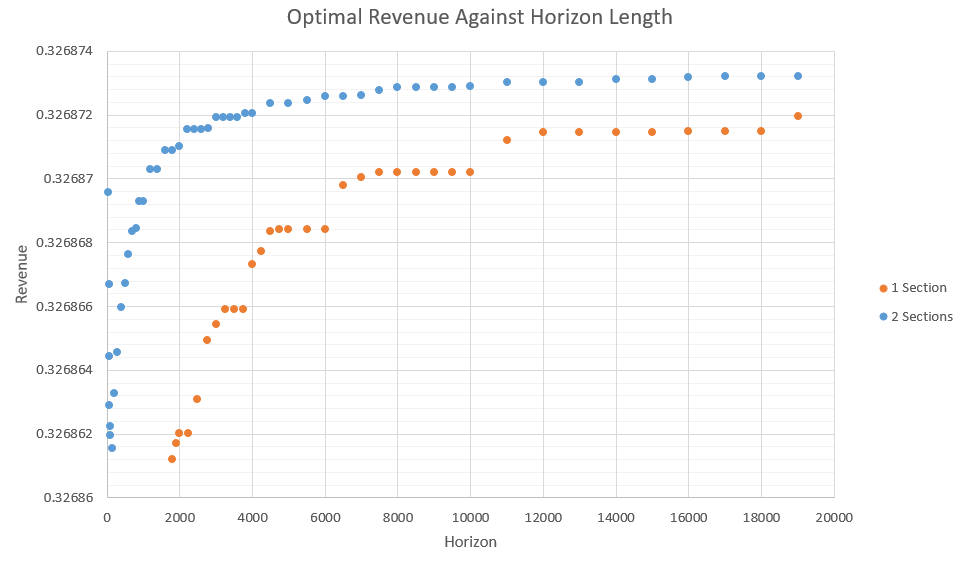
\includegraphics[width=\textwidth]{graph1.png}
    \caption{The method's results for Bitcoin with a $\alpha = 0.3, \gamma = 0.5$ and limiting the maximum fork length to 20}
    \label{fig:empirical_results}
\end{figure}

\subsection{Maximal Fork Length}
TODO: Graph for max fork
Show that this is negligible for fork > 20

\section{Discussion and Future Work}
TODO: Add to discussion
In addition to finding an approximately optimal policy, Sapirshtein's analysis provided an upper bound to the optimal revenue for any possible policy which takes into consideration policies which allow a maximum fork length of more than what truncation they used for their MDP. However their upper bound is not tight so it does not provide much information since using it for bounding the security threshold wouldn't yield accurate results.
In this paper the policy space is assumed to be the same for both the original MDP and the MDP obtained by the method and there is no reference to the actual upper bound when considering policies which allow very long forks. This is ignored since the probability of the attacker obtaining a very large fork declines exponentially with the fork length. Therefore, taking into consideration a large enough maximum fork length such as 100 is enough and increasing it fourther is negligible as shown in section \ref{Maximal Fork Length}.

SquirRL's method (\cite{hou2019squirrl}) is based on Sapirshtein's method (\cite{sapirshtein2016optimal}). They use approximated Q-learning instead of using value iteration to solve the MDP at every stage of the binary search. Approximated Q-learning gives much worse approximation than value iteration and is also stochastic. This interferes with the binary search and gives limits the results to be less accurate. Using the novel method with approximated Q-learning may reduce the error only to the approximation error of the function approximation used instead of both that and the stochastic nature of the method which interferes with the binary search.

\section{Conclusion}
TODO: Conclusion

\bibliographystyle{alpha}
\bibliography{refs}

\end{document}
